\chapter{}
Zur Motivation betrachten wir zur Einleitung in die letzte Vorlesung ein kleines Bildchen.
\begin{center}

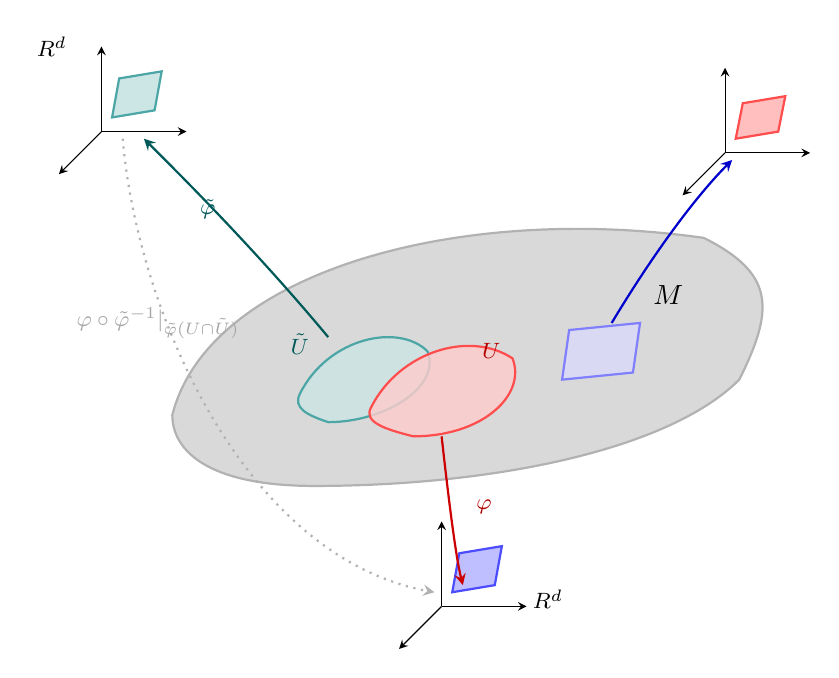
\begin{tikzpicture}[>=stealth, font=\small, scale= 0.9]

% ============================================================
% MANNIGFALTIGKEIT M (geschwungene Fläche)
% ============================================================
\fill[gray!30, opacity=1]
  (1.0, 1.5)
  .. controls (1.5, 3.5) and (5.0, 4.5) ..
  (8.5, 4.0)
  .. controls (9.5, 3.5) and (9.5, 3.0) ..
  (9.0, 2.0)
  .. controls (8.0, 1.0) and (5.5, 0.5) ..
  (3.0, 0.5)
  .. controls (1.5, 0.5) and (1.0, 1.0) ..
  cycle;

% Vorderkante (geschwungen, dicker)
\draw[gray!60, thick]
 (1.0, 1.5)
  .. controls (1.5, 3.5) and (5.0, 4.5) ..
  (8.5, 4.0)
  .. controls (9.5, 3.5) and (9.5, 3.0) ..
  (9.0, 2.0)
  .. controls (8.0, 1.0) and (5.5, 0.5) ..
  (3.0, 0.5)
  .. controls (1.5, 0.5) and (1.0, 1.0) ..
  cycle;

\node[font=\normalsize] at (8.0, 3.2) {$M$};

% ============================================================
% KARTE ~U (blau-grün, links, mit Überlappung)
% ============================================================
\fill[teal!20, opacity=0.8]
  (2.8, 1.8) .. controls (3.2, 2.6) and (4.2, 2.8) ..
  (4.6, 2.4) .. controls (4.8, 1.9) and (4.0, 1.4) ..
  (3.2, 1.4) .. controls (2.9, 1.5) and (2.7, 1.6) .. cycle;
\draw[teal!70, thick]
  (2.8, 1.8) .. controls (3.2, 2.6) and (4.2, 2.8) ..
  (4.6, 2.4) .. controls (4.8, 1.9) and (4.0, 1.4) ..
  (3.2, 1.4) .. controls (2.9, 1.5) and (2.7, 1.6) .. cycle;
\node[teal!70!black, font=\footnotesize] at (2.8, 2.5) {$\tilde{U}$};

% KARTE U (red, überlappt mit ~U)
\fill[red!20, opacity=0.8]
  (3.8, 1.6) .. controls (4.2, 2.4) and (5.2, 2.7) ..
  (5.8, 2.3) .. controls (6.0, 1.8) and (5.4, 1.2) ..
  (4.4, 1.2) .. controls (4.0, 1.3) and (3.7, 1.4) .. cycle;
\draw[red!70, thick]
  (3.8, 1.6) .. controls (4.2, 2.4) and (5.2, 2.7) ..
  (5.8, 2.3) .. controls (6.0, 1.8) and (5.4, 1.2) ..
  (4.4, 1.2) .. controls (4.0, 1.3) and (3.7, 1.4) .. cycle;
\node[red!70!black, font=\footnotesize] at (5.5, 2.4) {$U$};

% KARTE disjunkt (blau, rechts)
\fill[blue!15, opacity=0.7]
  (6.5, 2.0) -- (7.5, 2.1) -- (7.6, 2.8) -- (6.6, 2.7) -- cycle;
\draw[blue!50, thick]
  (6.5, 2.0) -- (7.5, 2.1) -- (7.6, 2.8) -- (6.6, 2.7) -- cycle;

% ============================================================
% KOORDINATENSYSTEM OBEN LINKS  R^d  (Bild von ~phi)
% ============================================================
\draw[->] (0.0, 5.5) -- (1.2, 5.5);
\draw[->] (0.0, 5.5) -- (0.0, 6.7);
\draw[->] (0.0, 5.5) -- (-0.6, 4.9);
\node[font=\footnotesize] at (-0.7, 6.7) {$\mathbb{R}^d$};
% red Parallelogramm
\fill[teal!20]
  (0.15, 5.7) -- (0.75, 5.8) -- (0.85, 6.35) -- (0.25, 6.25) -- cycle;
\draw[teal!70, thick]
  (0.15, 5.7) -- (0.75, 5.8) -- (0.85, 6.35) -- (0.25, 6.25) -- cycle;

% ============================================================
% KOORDINATENSYSTEM OBEN RECHTS  R^d  (Bild von phi)
% ============================================================
\draw[->] (8.8, 5.2) -- (10.0, 5.2);
\draw[->] (8.8, 5.2) -- (8.8,  6.4);
\draw[->] (8.8, 5.2) -- (8.2,  4.6);
% red Parallelogramm
\fill[red!25]
  (8.95, 5.4) -- (9.55, 5.5) -- (9.65, 6.0) -- (9.05, 5.9) -- cycle;
\draw[red!70, thick]
  (8.95, 5.4) -- (9.55, 5.5) -- (9.65, 6.0) -- (9.05, 5.9) -- cycle;

% ============================================================
% KOORDINATENSYSTEM UNTEN MITTE  R^d  (Bild von phi)
% ============================================================
\draw[->] (4.8, -1.2) -- (6.0, -1.2);
\draw[->] (4.8, -1.2) -- (4.8,  0.0);
\draw[->] (4.8, -1.2) -- (4.2, -1.8);
\node[font=\footnotesize] at (6.3, -1.1) {$\mathbb{R}^d$};
% red Parallelogramm
\fill[blue!25]
  (4.95, -1.0) -- (5.55, -0.9) -- (5.65, -0.35) -- (5.05, -0.45) -- cycle;
\draw[blue!70, thick]
  (4.95, -1.0) -- (5.55, -0.9) -- (5.65, -0.35) -- (5.05, -0.45) -- cycle;

% ============================================================
% PFEILE VON M
% ============================================================

% ~phi: von ~U nach oben links
\draw[->, teal!70!black, thick]
  (3.2, 2.6) .. controls (2.2, 3.8) and (1.2, 4.8) .. (0.6, 5.4);
\node[teal!70!black, font=\footnotesize] at (1.5, 4.4) {$\tilde{\varphi}$};

% phi: von U nach unten mitte
\draw[->, red!80!black, thick]
  (4.8, 1.2) .. controls (4.9, 0.3) and (5.0, -0.5) .. (5.1, -0.9);
\node[red!70!black, font=\footnotesize] at (5.4, 0.2) {$\varphi$};

% phi: von disjunkter Karte nach oben rechts
\draw[->, blue!80!black, thick]
  (7.2, 2.8) .. controls (7.8, 3.8) and (8.4, 4.6) .. (8.9, 5.1);

% ============================================================
% TRANSITIONSFUNKTION (gestrichelter Bogen unten links)
% ============================================================
\draw[->, dotted, thick, gray!60]
  (0.3, 5.4)
  .. controls (0.5, 3.0) and (2.0, -0.5) ..
  (4.7, -1.0);
\node[font=\footnotesize, gray!70, align=left] at (0.8, 2.8)
  {$\varphi \circ \tilde{\varphi}^{-1}|_{\tilde{\varphi}(U \cap \tilde{U})}$};

\end{tikzpicture}
\end{center}

Das Bild zeigt eine Mannigfaltigkeit $M$ (grau) mit drei Karten: $\tilde{U}$ (blau-grün), $U$ (red) und eine disjunkte Karte (blau). Die Karten $\tilde{U}$ und $U$ überlappen sich, und die Übergangsfunktion zwischen diesen beiden Karten ist als gestrichelter Bogen dargestellt. Die Pfeile zeigen die Kartenabbildungen $\tilde{\varphi}$
und $\varphi$ von den jeweiligen Karten in $\mathbb{R}^d$.  Lokal betrachtet sieht die Mannigfaltigkeit $M$
also wie $\mathbb{R}^d$ aus, aber global kann sie eine viel kompliziertere Struktur haben. 
Beispiele aus der echten Welte: Die Oberfläche der Erde, die Oberfläche eines Donuts, die Raumzeit 
in der Relativitätstheorie, die Konfigurationsräume von physikalischen Systemen, die Mannigfaltigkeit 
der Zustände in der Quantenmechanik, ... aber  auch die Menge der Lösungen einer Differentialgleichung, 
die Menge der Möglichkeiten, wie sich ein Roboter bewegen kann, die Menge der Bilder eines neuronalen
Netzes, ...
Aber damit genug von der Realität, zurück zur schönen und weniger Angst einflößenden Welt der Mathematik.

\dfn{Karte, Atlas} 
{
    Sei $\langle M, \mathcal{T}$ ein Topologischer Raum, $d \in \mathbb{N}$.
    \begin{itemize}
        \item[(i)] Ein paar $\langle U, \varphi \rangle$ heißt d-dimensionale 
        \textbf{Karte} 
        auf M $:\Leftrightarrow$
        \begin{itemize}
            \item $U \subseteq M$ offen
            \item $\varphi: U \to \mathbb{R}^d$ 
            \item $\varphi(U)$ offen in $\mathbb{R}^d$ mit Spurtopologie $\mathbb{R}^d$
            \item $\varphi: U \to \varphi(U)$ ist ein Homöomorphismus von $U$ 
            auf $\varphi(U)$ mit der Spurtopologie von $M$
        \end{itemize}
        \item[(ii)] Eine Familie 
        $\mathcal{A}:= \{\langle U_i, \varphi_i \rangle\}_{i \in I}$ 
        heißt d-dimensionaler \textbf{Atlas} von $M$, 
        $:\Leftrightarrow$
        \begin{itemize}
            \item $\forall i \in I:\langle U_i, \varphi_i \rangle$ 
            ist eine d-dimensionale Karte auf $M$
            \item $\forall i,j \in I$ mit $U_i \cap U_j \neq \emptyset$: 
            $\varphi_j \circ \varphi_i^{-1}|_{\varphi_i(U_i \cap U_j)}$ ist $C^1$ (Kartenwechsel)
            \item $\bigcup_{i \in I} U_i = M$ (die Karten überdecken $M$)
        \end{itemize}
    \end{itemize}
}
\dfn{$C^1$-Manigfaltigkeit}
{
Sei $d \in \mathbb{N}$ dann heißt $(\langle M, \mathcal{T} \rangle,\mathcal{A})$
eine \textbf{ $d$-dimensionale $C^1$-Mannigfaltigkeit}$:\Leftrightarrow$.
\begin{itemize}
    \item $\langle M, \mathcal{T} \rangle$ ist ein topologischer Raum
    \item es gibt eine höchstens abzählbare basis $\mathcal{B}$ von 
    $\mathcal{T}$, d.h. $\forall U \in \mathcal{T} \exists B \in \mathcal{B}:$ 
    $B \subseteq U$
    \item $\mathcal{A}$ ist ein d-dimensionaler Atlas von $M$
\end{itemize}
}
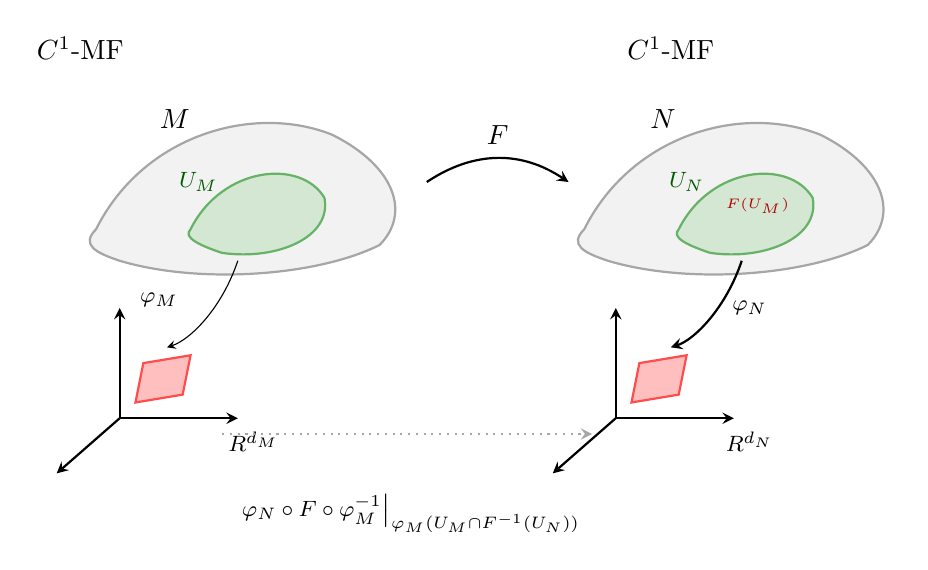
\begin{tikzpicture}[>=stealth, font=\small, scale=1.0]

% ============================================================
% TITEL
% ============================================================
\node[font=\normalsize] at (0.0, 6.5) {$C^1$-MF};
\node[font=\normalsize] at (7.5, 6.5) {$C^1$-MF};

% ============================================================
% LINKE MANNIGFALTIGKEIT M (Schirm-Form)
% ============================================================
\fill[gray!10]
  (0.2, 4.2)
  .. controls (0.8, 5.4) and (2.2, 5.8) ..
  (3.2, 5.4)
  .. controls (4.0, 5.0) and (4.2, 4.4) ..
  (3.8, 4.0)
  .. controls (3.0, 3.6) and (1.5, 3.5) ..
  (0.5, 3.8)
  .. controls (0.2, 3.9) and (0.0, 4.0) ..
  cycle;
\draw[gray!70, thick]
  (0.2, 4.2)
  .. controls (0.8, 5.4) and (2.2, 5.8) ..
  (3.2, 5.4)
  .. controls (4.0, 5.0) and (4.2, 4.4) ..
  (3.8, 4.0)
  .. controls (3.0, 3.6) and (1.5, 3.5) ..
  (0.5, 3.8)
  .. controls (0.2, 3.9) and (0.0, 4.0) ..
  cycle;
\node[font=\normalsize] at (1.2, 5.6) {$M$};

% Karte U_M auf M
\fill[Green!20, opacity=0.8]
  (1.4, 4.2) .. controls (1.8, 5.0) and (2.8, 5.1) ..
  (3.1, 4.6) .. controls (3.2, 4.1) and (2.5, 3.8) ..
  (1.8, 3.9) .. controls (1.5, 4.0) and (1.3, 4.1) .. cycle;
\draw[Green!60, thick]
  (1.4, 4.2) .. controls (1.8, 5.0) and (2.8, 5.1) ..
  (3.1, 4.6) .. controls (3.2, 4.1) and (2.5, 3.8) ..
  (1.8, 3.9) .. controls (1.5, 4.0) and (1.3, 4.1) .. cycle;
\node[Green!70!black, font=\footnotesize] at (1.5, 4.8) {$U_M$};

% ============================================================
% KOORDINATENSYSTEM LINKS UNTEN  R^{d_M}
% ============================================================
\draw[->, black, thick] (0.5, 1.8) -- (2.0, 1.8);
\draw[->, black, thick] (0.5, 1.8) -- (0.5, 3.2);
\draw[->, black, thick] (0.5, 1.8) -- (-0.3, 1.1);
\node[font=\footnotesize, black] at (2.2, 1.5) {$\mathbb{R}^{d_M}$};

% red Parallelogramm
\fill[red!25]
  (0.7, 2.0) -- (1.3, 2.1) -- (1.4, 2.6) -- (0.8, 2.5) -- cycle;
\draw[red!70, thick]
  (0.7, 2.0) -- (1.3, 2.1) -- (1.4, 2.6) -- (0.8, 2.5) -- cycle;

% Pfeil phi_M von Karte nach unten
\draw[->, black]
  (2.0, 3.8) .. controls (1.8, 3.2) and (1.4, 2.8) .. (1.1, 2.7);
\node[black, font=\footnotesize] at (1.0, 3.3) {$\varphi_M$};

% ============================================================
% PFEIL F  (Mitte, von M nach N)
% ============================================================
\draw[->, thick]
  (4.4, 4.8) .. controls (5.0, 5.2) and (5.6, 5.2) .. (6.2, 4.8);
\node[font=\normalsize] at (5.3, 5.4) {$F$};

% ============================================================
% RECHTE MANNIGFALTIGKEIT N (Schirm-Form)
% ============================================================
\fill[gray!10]
  (6.4, 4.2)
  .. controls (7.0, 5.4) and (8.4, 5.8) ..
  (9.4, 5.4)
  .. controls (10.2, 5.0) and (10.4, 4.4) ..
  (10.0, 4.0)
  .. controls (9.2, 3.6) and (7.7, 3.5) ..
  (6.7, 3.8)
  .. controls (6.4, 3.9) and (6.2, 4.0) ..
  cycle;
\draw[gray!70, thick]
  (6.4, 4.2)
  .. controls (7.0, 5.4) and (8.4, 5.8) ..
  (9.4, 5.4)
  .. controls (10.2, 5.0) and (10.4, 4.4) ..
  (10.0, 4.0)
  .. controls (9.2, 3.6) and (7.7, 3.5) ..
  (6.7, 3.8)
  .. controls (6.4, 3.9) and (6.2, 4.0) ..
  cycle;
\node[font=\normalsize] at (7.4, 5.6) {$N$};

% Karte U_N auf N
\fill[Green!20, opacity=0.8]
  (7.6, 4.2) .. controls (8.0, 5.0) and (9.0, 5.1) ..
  (9.3, 4.6) .. controls (9.4, 4.1) and (8.7, 3.8) ..
  (8.0, 3.9) .. controls (7.7, 4.0) and (7.5, 4.1) .. cycle;
\draw[Green!60, thick]
  (7.6, 4.2) .. controls (8.0, 5.0) and (9.0, 5.1) ..
  (9.3, 4.6) .. controls (9.4, 4.1) and (8.7, 3.8) ..
  (8.0, 3.9) .. controls (7.7, 4.0) and (7.5, 4.1) .. cycle;
\node[Green!70!black, font=\footnotesize] at (7.7, 4.8) {$U_N$};
% F(U_M) label
\node[red!70!black, font=\tiny] at (8.6, 4.5) {$F(U_M)$};

% ============================================================
% KOORDINATENSYSTEM RECHTS UNTEN  R^{d_N}
% ============================================================
\draw[->, black, thick] (6.8, 1.8) -- (8.3, 1.8);
\draw[->, , thick] (6.8, 1.8) -- (6.8, 3.2);
\draw[->, black, thick] (6.8, 1.8) -- (6.0, 1.1);
\node[font=\footnotesize, black] at (8.5, 1.5) {$\mathbb{R}^{d_N}$};

% red Parallelogramm
\fill[red!25]
  (7.0, 2.0) -- (7.6, 2.1) -- (7.7, 2.6) -- (7.1, 2.5) -- cycle;
\draw[red!70, thick]
  (7.0, 2.0) -- (7.6, 2.1) -- (7.7, 2.6) -- (7.1, 2.5) -- cycle;

% Pfeil phi_N von Karte nach unten
\draw[->, black, thick]
  (8.4, 3.8) .. controls (8.2, 3.2) and (7.8, 2.8) .. (7.5, 2.7);
\node[black, font=\footnotesize] at (8.5, 3.2) {$\varphi_N$};

% ============================================================
% GESTRICHELTER PFEIL UNTEN (Transitionsfunktion)
% ============================================================
\draw[->, dotted, thick, gray!70]
  (1.8, 1.6) -- (6.5, 1.6);

% Label Transitionsfunktion
\node[font=\footnotesize, align=center] at (4.2, 0.6)
  {$\varphi_N \circ F \circ \varphi_M^{-1}\big|_{\varphi_M(U_M \cap F^{-1}(U_N))}$};

\end{tikzpicture}

\dfn{$C^1$ Funktion zwischen Mannigfaltigkeiten}
{
    Seien $(\langle M, \mathcal{T} \rangle, \mathcal{A})(\langle N, \mathcal{V}\rangle, \mathcal{B})$ 
    mit 
    $\mathcal{A} := \{\langle U_{M,i}, \varphi_{M,i} \rangle \mid i \in I\}$ und
    $\mathcal{B}:= \{\langle U_{N,j}, \varphi_{N,j} \rangle \mid j \in J\}$
    dann heißt eine Funktion $F: M \to N$
\textbf{$C^1$-Funktion} $:\Leftrightarrow$
\begin{itemize}
    \item $F$ ist stetig
    \item $\forall x \in M \forall i \in I$ mit $x \in U_n,i$
    $\forall j \in J$ mit $F(x) \in U_{N,j}$:
    $$\varphi_{N,j} \circ F \circ \varphi_{M,i}^{-1}\big|_{\varphi_{M,i}
    (U_{M,i} \cap F^{-1}(U_{N,j}))}
    $$ ist eine $C^1$-Funktion von $\varphi_{M,i}(U_{M,i} \cap F^{-1}(U_{N,j}))$
    nach $\varphi_{N,j}(U_{N,j})$.
\end{itemize}   
}
\mlenma{}
{
    Sei $(\langle M, \mathcal{T} \rangle, \mathcal{A})$ eine $C^1$-Mannigfaltigkeit.
    Dann ist $id:M\to N$ eine $C^1$-Funktion. 
}
\begin{proof}{Lemma: 13.0.4}
    Sei $x \in M$ Sei $i \in I$ und $x \in \mathcal{U}_i$. Sei $j \in I$
    mit $id(x)=x \in \mathcal{U}_j$.\\
    $\mathcal{A}:=\{(\mathcal{U}_i, \varphi_i) \mid i \in I\}$\\
    $$ \varphi_j \circ id_M \circ \varphi_i^{-1}\big|_{\varphi_i(\mathcal{U}_i \cap id_M^{-1}(\mathcal{U}_j))}=
    \varphi_j \circ \varphi_i^{-1}\big|_{\varphi_i(\mathcal{U}_i \cap \mathcal{U}_j)} \in C^1
    $$
\end{proof}

wobei gilt
\begin{tikzcd} 
M \arrow[r, "F"] \arrow[rr, bend right, "G \circ F"'] & N 
\arrow[r, "G"] & L
\end{tikzcd} 
$M, N, L \in \mathcal{C}^1\text{-MF}, \ F, G \in \mathcal{C}^1 
\Rightarrow G \circ F \in \mathcal{C}^1$


\dfn{Diffeomorphismus}
{
    M,N $C^1$-Mannigfaltigkeiten, $F: M \to N$ heißt 
    \textbf{Diffeomorphismus}$:\Leftrightarrow$
    \begin{itemize}
        \item $F$ ist Homöomorphismus von $M$ auf $N$
        \item $F$ und $F^{-1}$ sind $C^1$-Funktionen
    \end{itemize}
}

\nt{
    \begin{itemize}
        \item Sei $\langle M, \mathcal{T}\rangle$ ein topologischer Raum, 
        dann kann es $\mathcal{A},\mathcal{A'}$ atlanten geben, so dass
        $id_m$ ist nihct Diffeomorphismus von 
        $(\langle M, \mathcal{T} \rangle, \mathcal{A})$ 
        auf $(\langle M, \mathcal{T} \rangle, \mathcal{A'})$.
        \item Ist $(\langle M, \mathcal{T} \rangle, \mathcal{A})$ 
        eine $C^1$-Mannigfaltigkeit, 
        $\Rightarrow \{\mathcal{A'}\mid \mathcal{A'}C^1\}$-Atlas auf
         $M$ mit $id_M$ ist Diffeomorphismus von 
         $(\langle M, \mathcal{T} \rangle, \mathcal{A})\to
         (\langle M, \mathcal{T} \rangle, \mathcal{A'})$.
         Hat größtes Element
    \end{itemize}
}

\ex{}
{
Sei $M\subseteq \mathbb{R}^d$ offen, $\mathcal{T}:=$Spurtopologie auf $M$
von der Euklidischen Topologie auf $\mathbb{R}^d$,
$\mathcal{A}:=\{\langle M, \iota_M \rangle\}$ wobei 
$$
\iota_M:\begin{cases} M \to \mathbb{R}^d, \\ x \mapsto x \end{cases}
$$
\begin{itemize}
  \item $\left\{ \prod_{i=1}^d (a_i, b_i) \;\middle|\; a_i, b_i \in \mathbb{Q} \right\}$
        ist Basis d. euklid. Top. u. abzb.

  \medskip
  $\Rightarrow \left\{ M \cap \prod_{i=1}^d (a_i, b_i) \;\middle|\; a_i, b_i \in \mathbb{Q} \right\}$
  ist Basis der Spurtop. auf $M$

  \item $M$ offen in $M$,\quad $\iota_M : M \to \mathbb{R}^d$,\quad
        $\iota_M(M) = M$ offen in $\mathbb{R}^d$

  $\iota_M : \langle M,\, \mathcal{E}|_M \rangle \to \langle M,\, \mathcal{E}|_M \rangle$
  \quad Homöom.

  also $(M, \iota_M)$ ist Karte

  \item ,,Kartenwechsel``\quad
        $\iota_M \circ \iota_M^{-1}\big|_{\iota_M(M \cap M)} = \mathrm{id}_M$
        \quad ist $C^\infty$

  \item $\bigcup_{\text{Karten}} = M$
\end{itemize}


\begin{center}
\begin{tikzpicture}[scale=1.0,
  axis/.style={-{Stealth[length=3.5pt]}, thin, opacity=0.7},
]

% ===== Koordinatensystem =====
\draw[axis] (0,0) -- (4.5, 0)    node[right] {$x_1$};
\draw[axis] (0,0) -- (0, 4.5)    node[above] {$x_3$};
\draw[axis] (0,0) -- (-1.4,-1.1) node[below left] {$x_2$};

% Ursprung
\fill (0,0) circle (1.5pt);
\node[below right, font=\scriptsize] at (0,0) {$O$};

% ===== Linke Ellipse: M =====
\draw[fill=blue!8, draw=blue!50!black, thick]
  (0.9, 1.8) ellipse (0.75 and 1.05);
\draw[fill=blue!18, draw=none]
  (0.85, 1.85) ellipse (0.44 and 0.64);
\node[blue!40!black, font=\bfseries] at (0.9, 1.8) {$M$};

% ===== Rechte Ellipse: M in R^d =====
\draw[fill=green!8, draw=green!40!black, thick]
  (3.4, 1.8) ellipse (0.75 and 1.05);
\draw[fill=green!18, draw=none]
  (3.35, 1.85) ellipse (0.44 and 0.64);
\node[green!30!black, font=\bfseries] at (3.4, 1.8) {$M$};

% R^d Label
\node[black, font=\small\bfseries] at (4.4, 4.0)
  {$\mathbb{R}^d$};

% ===== Pfeil iota_M =====
\draw[
  -{Stealth[length=5pt]},
  black, thick,
  bend left=25
]
(1.68, 2.55) to
  node[above, font=\small] {$\iota_M$}
(2.62, 2.55);

\end{tikzpicture}
\end{center}
}
\ex{}
{
  Sei 
  $$
  M:=\left\{ \begin{pmatrix} x_1 \\ x_2 \\ x_3 \end{pmatrix} \in \mathbb{R}^3 \;\middle|\; x_1^2 + x_2^2 + x_3^2 = 1 \right\} =: S^2
  \qquad \text{\textit{nicht offen!}}
  $$
  mit der Spurtopologie $\mathcal{T}$ auf $\mathbb{R}^3$ 

\begin{center}
\begin{tikzpicture}[scale=1.8,
  axis/.style={-{Stealth[length=5pt]}, thick},
  meridian/.style={gray!60, thin},
  sphere/.style={draw=blue!70!blue, fill=blue!15, fill opacity=0.7}
]

% 3D perspective offset
\def\ax{0.55}  % x1-axis x-component
\def\ay{-0.3}  % x1-axis y-component
\def\bx{-0.55} % x2-axis x-component
\def\by{-0.3}  % x2-axis y-component

% Base disk (flat bottom of hemisphere)
\draw[fill=blue!8, draw=blue!50, thin]
  (0,0) ellipse (1 and 0.28);

% Grid lines on base disk
\draw[blue!30, very thin] (-1,0) -- (1,0);
\draw[blue!30, very thin] (0,-0.28) -- (0,0.28);

% Latitude rings on hemisphere (dashed)
\draw[meridian, dashed]
  (0,0.5) ellipse (0.866 and 0.242);
\draw[meridian, dashed]
  (0,0.866) ellipse (0.5 and 0.14);

% Meridian lines (vertical) dashed back
\draw[meridian, dashed]
  (0,1) arc[start angle=90, end angle=270, x radius=0.28, y radius=1];

% Hemisphere fill + front outline
\begin{scope}
  \clip (-1.1,-0.01) rectangle (1.1,1.1);
  \draw[sphere, line width=1.2pt]
    (-1,0) arc[start angle=180, end angle=0, x radius=1, y radius=1] -- cycle;
\end{scope}

% Front meridian
\draw[blue!60, thin]
  (0,1) arc[start angle=90, end angle=-90, x radius=0.28, y radius=1];

% Front equator arc (solid)
\draw[blue!80, line width=1.5pt]
  (-1,0) arc[start angle=180, end angle=0, x radius=1, y radius=0.28];

% Back equator (dashed)
\draw[blue!50, dashed, thin]
  (-1,0) arc[start angle=180, end angle=360, x radius=1, y radius=0.28];

% ---- Coordinate axes ----
\draw[axis] (0,0) -- (1.6*\ax, 1.6*\ay) node[right] {$x_1$};
\draw[axis] (0,0) -- (1.6*\bx, 1.6*\by) node[left]  {$x_2$};
\draw[axis] (0,0) -- (0, 1.45)           node[above] {$x_3$};

% Origin
\fill (0,0) circle (1.5pt);
\node[below right, font=\small] at (0,0) {$O$};

% North pole
\fill[blue!80!blue] (0,1) circle (2pt);

% Sphere label
\node[blue!70!blue, font=\small\itshape] at (1.15, 0.7) {$M = S^2$};
\draw[blue!50, dashed, very thin] (0.95,0.68) -- (0.72, 0.72);

% Radius label
\draw[blue!40, dashed] (0,0) -- (0.707, 0.707);
\node[blue!60, font=\scriptsize] at (0.43, 0.45) {$1$};

% Point on sphere
\fill[orange] (0.7, 0.714) circle (2pt);
\node[orange!80!black, font=\scriptsize, right] at (0.72,0.71) {$P \in M$};

% nicht offen annotation
\node[gray, font=\small\itshape] at (1.7, 1.1) {\textit{nicht offen!}};

\end{tikzpicture}
\end{center}

für alle $j\in \{1,2,3\}$ sei 
$$
  U_{j+}:=\left\{ \begin{pmatrix} x_1 \\ x_2 \\ x_3 \end{pmatrix} 
  \in M \;\middle|\; x_j > 0 \right\}, \quad \phi_{\epsilon +}:U_{\epsilon +} 
  \to \mathbb{D}:=\{(a,b) \in \mathbb{R}^2 \mid a^2 + b^2 < 1\}, \quad
  \begin{pmatrix} x_1 \\ x_2 \\ x_3 \end{pmatrix} \mapsto 
  \begin{pmatrix} x_1\\ x_2 \end{pmatrix}
$$
$$
  U_{j-}:=\left\{ \begin{pmatrix} x_1 \\ x_2 \\ x_3 \end{pmatrix} 
  \in M \; \middle|\; x_j < 0 \right\},\quad \phi_{\epsilon -}:U_{\epsilon -} \to  
  \mathbb{D}:=\{(a,b) \in \mathbb{R}^2 \mid a^2 + b^2 < 1\}, \quad
  \begin{pmatrix} x_1 \\ x_2 \\ x_3 \end{pmatrix} \mapsto \begin{pmatrix} x_2\\ x_3 \end{pmatrix}
$$
$\phi_{y\pm}:\dots$ Analog\\
$\mathcal{A}:=\{(U_{1+}, \phi_{1+}), (U_{1-}, \phi_{1-}), (U_{2+}, \phi_{2+}), (U_{2-}, \phi_{2-}), (U_{3+}, \phi_{3+}), (U_{3-}, \phi_{3-})\}$
\begin{itemize}
  \item Sei $\begin{pmatrix} x_1 \\ x_2 \\ x_3 \end{pmatrix} \in M \Rightarrow x_1^2 + x_2^2 + x_3^2 = 1 \Rightarrow$
        $\begin{pmatrix} x_1 \\ x_2 \end{pmatrix} \neq 0$
        Wähle $j:x_j \neq 0 $
        $$
        \begin{cases}
          x_j > 0 \Rightarrow U_{j+} \\
          x_j < 0 \Rightarrow U_{j-}
        \end{cases}
    $$
    also $\bigcup_{j=1,2,3} (U_{j+} \cup U_{j-}) = M$
  \item $(U_{1-}, \phi_{1-})$ ist Karte auf $M$:
  $U_{1-}=M\cap \{\begin{pmatrix}
x_1 \\ x_2 \\ x_3 \end{pmatrix} \in \mathbb{R}^3 \mid x_1 < 0\}
  \Rightarrow U_{1-}$ offen in $M$ mit Spurtopologie

  \begin{center}
\begin{tikzpicture}[scale=1.7,
  axis/.style={-{Stealth[length=4pt]}, thick},
]

% ---- Sphere ----
% Gray sphere fill
\draw[fill=gray!10, draw=none] (0,0) circle (1);

% Orange left hemisphere patch (x1 < 0)
\begin{scope}
  \clip (-1.05,-1.05) rectangle (0,1.05);
  \draw[fill=orange!40, draw=none] (0,0) circle (1);
\end{scope}
\draw[orange!70!red, fill=orange!30, fill opacity=0.6]
  (0,1) arc[start angle=90, end angle=270,
            x radius=0.28, y radius=1]
  arc[start angle=270, end angle=90,
            x radius=1, y radius=1];

% Back equator dashed
\draw[gray!50, dashed, thin]
  (1,0) arc[start angle=0, end angle=180, x radius=1, y radius=0.28];

% Sphere outline
\draw[black!70, thick] (0,0) circle (1);

% Front equator
\draw[black!60]
  (-1,0) arc[start angle=180, end angle=0, x radius=1, y radius=0.28];

% Left meridian boundary (front)
\draw[orange!80!red, thick]
  (0,1) arc[start angle=90, end angle=270, x radius=0.28, y radius=1];
% Left meridian boundary (back, dashed)
\draw[orange!60!red, dashed]
  (0,1) arc[start angle=90, end angle=-90, x radius=0.28, y radius=1];

% Latitude rings (faint)
\draw[gray!40, very thin, dashed]
  (0,0.5) ellipse (0.866 and 0.242);
\draw[gray!40, very thin, dashed]
  (0,-0.5) ellipse (0.866 and 0.242);

% ---- Coordinate axes ----
\draw[axis] (-1.3,0)  -- (1.6,0)   node[right] {$x_1$};
\draw[axis] (0,-1.3)  -- (0,1.5)   node[above] {$x_3$};
\draw[axis] (0.2,-0.1)-- (-1.0,-0.5) node[below left] {$x_2$};

% Origin
\fill (0,0) circle (1.5pt);

% U_{1-} label
\node[orange!80!red, font=\small\bfseries] at (-1.3, 0.9) {$U_{1-}$};
\draw[orange!60!red, thin, dashed] (-1.15,0.85) -- (-0.55,0.55);

% x1 < 0 label
\node[orange!70!black, font=\scriptsize] at (-0.5,0) {$x_1\!<\!0$};

% ---- Mapping arrow ----
\draw[orange!80!red, -{Stealth[length=5pt]}, thick]
  (1.8, 0) -- (2.8, 0) node[midway, above, font=\small] {$\varphi_{1-}$};

% ---- D disk ----
\draw[fill=orange!15, draw=orange!70!red, thick]
  (3.5, 0) circle (0.55);
\node[orange!80!black, font=\small\bfseries] at (3.5, 0) {$D$};
\node[gray, font=\scriptsize] at (3.5, -0.75) {offen in $\mathbb{R}^2$};

% ---- Grid inside D ----
\draw[orange!30, very thin]
  (2.95,0) -- (4.05,0) (3.5,-0.55) -- (3.5,0.55);

\end{tikzpicture}
\end{center}
$$
  \varphi_{1-} : U_{1-} \to \mathbb{R}^d, \qquad \varphi_{1-}(U_{1-}) = D \text{ offen in } \mathbb{R}^d
$$
$$
  \varphi_{1-}\begin{pmatrix} x_1 \\ x_2 \\ x_3 \end{pmatrix} = \begin{pmatrix} x_2 \\ x_3 \end{pmatrix} \quad \text{stetig}
$$
$$
  \varphi_{1-}^{-1}\begin{pmatrix} s \\ t \end{pmatrix} = \begin{pmatrix} -\sqrt{1 - s^2 - t^2} \\ s \\ t \end{pmatrix} \quad \text{stetig}
$$
\item Kartenwechsel: 
\end{itemize}
}